%%%%%%%%%%%%%%%%%%%%%%%%%%%%%%%%%%%%%%%%%%%%%%%%%%%%%%%%%%%%%%%%%%%%%
%% Document Class
%%%%%%%%%%%%%%%%%%%%%%%%%%%%%%%%%%%%%%%%%%%%%%%%%%%%%%%%%%%%%%%%%%%%%
\documentclass[journal=jacsat,manuscript=article]{achemso}

%%%%%%%%%%%%%%%%%%%%%%%%%%%%%%%%%%%%%%%%%%%%%%%%%%%%%%%%%%%%%%%%%%%%%
%% Custom Commands
%%%%%%%%%%%%%%%%%%%%%%%%%%%%%%%%%%%%%%%%%%%%%%%%%%%%%%%%%%%%%%%%%%%%%
\newcommand*\mycommand[1]{\texttt{\emph{#1}}}
\newcommand{\al}{\textcolor{blue}}
\newcommand{\mz}{\textcolor{violet}}

%%%%%%%%%%%%%%%%%%%%%%%%%%%%%%%%%%%%%%%%%%%%%%%%%%%%%%%%%%%%%%%%%%%%%
%% Packages
%%%%%%%%%%%%%%%%%%%%%%%%%%%%%%%%%%%%%%%%%%%%%%%%%%%%%%%%%%%%%%%%%%%%%

%%% Chemistry
\usepackage[version=3]{mhchem}

%%% Graphics & Figures
\usepackage{graphicx}
\usepackage{float}
\usepackage{tikz}
\usetikzlibrary{shapes.geometric, arrows}

%%% Math
\usepackage{amsmath}
\usepackage{amssymb}
\usepackage{amsfonts}
\usepackage{amsthm}
\usepackage{mathrsfs}
\usepackage{mathtools}

%%% Tables
\usepackage{multirow}
\usepackage{booktabs}
\usepackage{tabularx}
\usepackage{makecell}

%%% Layout & Formatting
\usepackage{geometry}
\newgeometry{left=0.5in, right=0.5in, top=1in, bottom=1in}
\usepackage{calc}
\usepackage{xcolor}
\usepackage{textcomp}
\usepackage{soul}
\usepackage{ulem}
\usepackage[section]{placeins}

%%% Captions
\usepackage{caption}
\captionsetup[figure]{font=footnotesize}

%%% Appendix
\usepackage[title]{appendix}

%%% Algorithm  —  algorithm2e only (removes conflict with algorithm/algorithmicx/algpseudocode)
\usepackage[ruled,vlined,linesnumbered]{algorithm2e}

%%% Listings
\usepackage{listings}

%%% Footnotes
\usepackage{manyfoot}

%%% Hyperlinks & Cross-referencing
\usepackage{hyperref}
\usepackage{xr-hyper}
\usepackage{xr}
\usepackage{subfiles}
\ifdefined\SIbuild\else\externaldocument[S-]{SI}\fi


%%%%%=============================================================================%%%%
%%%%  Remarks: This template is provided to aid authors with the preparation
%%%%  of original research articles intended for submission to journals published 
%%%%  by Springer Nature. The guidance has been prepared in partnership with 
%%%%  production teams to conform to Springer Nature technical requirements. 
%%%%  Editorial and presentation requirements differ among journal portfolios and 
%%%%  research disciplines. You may find sections in this template are irrelevant 
%%%%  to your work and are empowered to omit any such section if allowed by the 
%%%%  journal you intend to submit to. The submission guidelines and policies 
%%%%  of the journal take precedence. A detailed User Manual is available in the 
%%%%  template package for technical guidance.
%%%%%=============================================================================%%%%

%% as per the requirement new theorem styles can be included as shown below
\theoremstyle{thmstyleone}%
\newtheorem{theorem}{Theorem}%  meant for continuous numbers
%%\newtheorem{theorem}{Theorem}[section]% meant for sectionwise numbers
%% optional argument [theorem] produces theorem numbering sequence instead of independent numbers for Proposition
\newtheorem{proposition}[theorem]{Proposition}% 
%%\newtheorem{proposition}{Proposition}% to get separate numbers for theorem and proposition etc.

\theoremstyle{thmstyletwo}%
\newtheorem{example}{Example}%
\newtheorem{remark}{Remark}%

\theoremstyle{thmstylethree}%
\newtheorem{definition}{Definition}%

\raggedbottom
%%\unnumbered% uncomment this for unnumbered level heads


\author{Awwal D. Oladipupo}
\affiliation[ChemE-UM]
{Department of Chemical Engineering, University of Michigan, 500 S State St., Ann Arbor, MI, USA, 48109}

\author{Dean M. Sweeney}
\affiliation[ChemE-UM]
{Department of Chemical Engineering, University of Michigan, 500 S State St., Ann Arbor, MI, USA, 48109}

\author{Roshini Dantuluri}
\affiliation[ChemE-UM]
{Department of Chemical Engineering, University of Michigan, 500 S State St., Ann Arbor, MI, USA, 48109}

\author{Bryan R. Goldsmith}
\affiliation[ChemE-UM]
{Department of Chemical Engineering, University of Michigan, 500 S State St., Ann Arbor, MI, USA, 48109}

\author{Rebecca K. Lindsey}
\affiliation[ChemE-UM]
{Department of Chemical Engineering, University of Michigan, 500 S State St., Ann Arbor, MI, USA, 48109}


\title[Article Title]{Bridging Film and Droplet Phenomena for Predicting Liquid Loading in Gas Wells with Machine Learning}

\begin{document}

%% Document Outline
%%=============================================================%%
%% 2 pages of introduction 
%% 2-3 pages of methods 
%%=============================================================%%
%%=============================================================%%
%% GivenName	-> \fnm{Joergen W.}
%% Particle	-> \spfx{van der} -> surname prefix
%% FamilyName	-> \sur{Ploeg}
%% Suffix	-> \sfx{IV}
%% \author*[1,2]{\fnm{Joergen W.} \spfx{van der} \sur{Ploeg} 
%%\sfx{IV}}\email{iauthor@gmail.com}
%%=============================================================%%

%%==================================%%
%% Sample for unstructured abstract %%
%%==================================%%
\newpage
\abstract{When extracting natural gas from wells, the gas velocity can fall below a critical threshold, leading to liquid accumulation in the tubing or casing---a phenomenon known as liquid loading. This issue limits sustained gas well production. Existing mechanistic descriptions are typically based on either droplet transport (Liquid Droplet Models, LDMs) or liquid film behavior (Liquid Film Models, LFMs), yet both struggle to capture the coupled physics governing real wellbore flows. We introduce a closed-form expression based on physical principles, with data used to estimate the unknown parameters, termed the Droplet Film Model (DFM). The DFM integrates mechanisms for liquid film and droplet transport to predict liquid loading across wellbore deviation angles. This model identifies the dominant flow mechanism through a film share evaluated with a fitted mixing parameter $\alpha$, and classifies wells as unloaded or loaded. \al{Because the true critical rate is never measured, the DFM parameters are learned directly from the observed well status, and a learned log-space residual corrects the physics-based critical rate. The DFM achieves a classification accuracy of 85.8\% $\pm$ 3.5\% (mean $\pm$ standard deviation over 5-fold cross-validation) and 90.9\% on the 44 held-out test wells.} To analyze predictive performance and interpretability, we compare DFM against two alternative approaches: the Qlattice symbolic regression method, which discovers interpretable equations from data, and the state-of-the-art tabular classifier TabPFN, representing a high-performance black-box baseline. \al{TabPFN achieves the highest cross-validation accuracy (91.8\% $\pm$ 4.7\%, compared with 82.4\% $\pm$ 5.2\% for QLattice), but all three models reach similar accuracy on the held-out test wells (DFM 90.9\%, QLattice 88.6\%, TabPFN 84.1\%). The six near-loaded wells were withheld from training and counted as loaded. DFM therefore attains predictive performance comparable to the black-box baseline while offering physically meaningful interpretability. Using the film share computed with the fitted global $\alpha$, the droplet term dominates the critical rate at all deviation angles in the data (20--90$^\circ$); the film contribution is largest at low deviation (median 30\% at 20--35$^\circ$) and is identically zero in horizontal wells.}}


%\keywords{ Liquid loading, symbolic ML, physics informed, liquid droplet, liquid film reversal }

%%\pacs[JEL Classification]{D8, H51}

%%\pacs[MSC Classification]{35A01, 65L10, 65L12, 65L20, 65L70}

\newpage 

\section{Introduction}\label{intro}

During natural gas extraction, upward gas flow exerts sufficient interfacial shear and drag to entrain liquid and transport it toward the surface. However, when the gas momentum becomes insufficient to overcome gravity and hydrostatic forces, liquid begins to fall back and accumulate in the wellbore. This accumulation of liquid is called liquid loading, and it is a major challenge for gas well production.\cite{CHEN2024205394, riza_pragmatic_2016, CHEN2016178}. This phenomenon creates hydrostatic backpressure that can exceed the formation pressure, restrict gas flow, and stop the desired production of gaseous hydrocarbons if left unmanaged. Ultimately, this detrimental process can lead to economic losses and costly operations to restore production. 

Accurate forecasting of liquid loading in gas wells would enable timely intervention to mitigate its consequences, such as temporarily shutting the well to allow pressure buildup or applying chemical treatments\cite{USEPA2011, Abhulimen}. Gas well production data typically include measurements such as flow rates, pressures, temperatures, and gas-liquid ratios. However, detecting liquid loading using this data alone is challenging because it does not directly measure liquid accumulation within the wellbore. Although production data can provide indirect indicators of loading, these signals are not unique and may also be influenced by factors such as gas-rate fluctuations, condensation, and multiphase flow transitions. Additionally, liquid loading often develops gradually, with its effects becoming apparent only after significant liquid accumulation, making early detection difficult without high-resolution downhole measurements of phase behavior (e.g., liquid holdup or phase flow rates). Therefore, developing a model that effectively captures the underlying physical phenomena occurring within a wellbore could enable more reliable prediction of liquid loading and effective mitigation\cite{Adaze2018, Adriana2019,Makinde2013}.

Liquid loading has often been analyzed using two mechanistic frameworks: droplet-based models (collectively referred to as Liquid Droplet Models, LDMs) and film-based models (Liquid Film Models, LFMs).\cite{Dukler1960} LDMs describe liquid as discrete droplets within the gas stream\cite{CHEN2016178, Chen2016}. In this framework, gas flow shears small liquid droplets from the wellbore wall and carries them upward. The effectiveness of this transport mechanism depends on factors such as gas velocity, droplet size, and surface tension. At sufficiently high gas velocities, the droplets remain suspended and are pushed to the surface. However, larger droplets may receive insufficient lift as the gas velocity decreases, causing them to fall back and accumulate\cite{Turner1969, Coleman1991a, Li2001}.

In contrast, LFMs describe liquid loading as a continuous film on the wellbore walls. The liquid film flows downward due to gravity, while the upward-moving gas applies shear forces to counteract this flow. The stability of this liquid film is crucial to determining whether liquid loading will occur. If the gas velocity is sufficiently high, the shear force exerted by the gas can keep the liquid film thin, preventing excessive accumulation. However, when the gas velocity falls below a critical threshold, the liquid film thickens, leading to an increased hydrostatic pressure that further restricts gas production. Researchers studying this approach focus on modeling the thickness, stability, and breakup of the liquid film to predict when and where liquid loading may occur\cite{Turner1969, Faidairo2014, LANDJOBOPAGOU2020103641}.  

Under their respective approaches and assumptions, these models determine the critical gas velocity or critical gas rate, which serves as a benchmark to assess the production status of a well. When the gas rate is below the critical rate, the well is classified as liquid-loaded. When the current gas rate is near the critical gas rate, the well is classified as near-loaded, meaning that it is approaching an unstable condition and may soon face liquid loading problems. Lastly, when the actual gas rate exceeds the critical rate, the well is considered unloaded, operating in a stable regime where gas flow is sufficient to carry liquids to the surface without hindering production.

Despite advances in LDMs and LFMs, their predictive reliability remains limited due to simplifying assumptions that do not fully capture the complex dynamics of multiphase flow in gas wells. LDMs typically assume that entrained liquid droplets are spherical or approximately ellipsoidal\cite{Turner1969, Coleman1991a, Coleman1991b, Coleman1991c, Nosseir2000, belfroid_prediction_2008, Li2001}. In practice, droplet shapes and sizes are highly variable and evolve dynamically due to coalescence and breakup processes, producing irregular droplet distributions\cite{Veeken2011}. Similarly, LFMs often assume that liquid forms a uniform film along the tubing wall\cite{KUMAR2017117}. However, film thickness can vary significantly along the wellbore due to pressure gradients, gas velocity changes, and surface roughness. Interfacial waves and disturbances frequently develop along the film surface, introducing instabilities and energy dissipation that are not captured by simplified theoretical descriptions.

In addition to these simplifying assumptions, existing models often neglect the influence of well geometry, pipe diameter, and operating conditions on liquid loading behavior.\cite{Barnea1980, LANDJOBOPAGOU2020103641}.  Experimental and field studies indicate that liquid holdup, liquid film thickness, and critical gas velocity exhibit non-monotonic dependence on wellbore inclination angle, with intermediate deviation angles often experiencing more severe loading than purely vertical or horizontal wells\cite{belfroid_prediction_2008, LANDJOBOPAGOU2020103641, Chen2016, Veeken2011, Luo2013}. In some systems, these effects peak at intermediate inclination angles of approximately 50–60°, reflecting a transition in flow behavior and the balance between liquid film buildup and droplet transport mechanisms. Also, larger-diameter wells tend to experience liquid loading earlier than smaller conduits. Altogether, these observations highlight that liquid loading arises from a complex interplay among droplet transport, liquid film dynamics, well geometry, and fluid properties\cite{WangY2010}.

Previous studies disagree on the dominant mechanism responsible for the onset of liquid loading. Some studies attribute the onset primarily to the behavior of the liquid film\cite{Veeken2011, Joseph2018, Waltrich2015}, whereas others suggest that it is governed by the dynamics of entrained liquid droplets\cite{KUMAR2017117, Liu2018, Veeken2011}. We hypothesize that both mechanisms contribute, with their relative importance depending on wellbore deviation. On this basis, we propose that integrating liquid droplet and liquid film reversal theories within a unified modeling framework can improve the prediction of critical gas conditions across a broad range of well geometries.

In this work, we construct and compare three distinct modeling paradigms to address the limitations of current models and accurately predict liquid loading behavior. The first is a physics-based model that explicitly incorporates a liquid droplet model and a liquid film model to represent the underlying physical processes. The second is a physics-informed symbolic learning framework, QLattice, in which physical structure and constraints guide the discovery of functional relationships from data. The third consists of a conventional black-box machine learning model (TabPFN) that infers system behavior directly from data without imposing explicit physical assumptions. In addition, we refine existing models by optimizing parameters reported in the literature and benchmark their performance against these three approaches. Through this comparative analysis, we assess the extent to which different modeling paradigms capture liquid loading behavior and examine the limitations of relying on any single framework.

\section{Methods}\label{sec:method}
We curated a dataset covering 208 wells with a range of operating conditions and classifications, including loaded, unloaded, near-loaded, and wells with uncertain loading status. Well information was collected from a variety of sources, and the curation process and the dataset are detailed in the Supplementary Information.  The dataset is imbalanced, comprising \al{75 loaded wells}, 111 unloaded wells, 6 near-loaded wells, and 16 uncertain wells. The initial feature set includes 32 variables that encompass both well characteristics (e.g., pipe diameter, deviation angle, and elevation) and flow-related properties (e.g., flow rates, densities, viscosities, Reynolds numbers, and film characteristics). A list of these features is provided in  \hl{Table-S1}. We began by acquiring and preprocessing the dataset, followed by exploratory data analysis, and subsequently developed a suite of ML models, as summarized in Figure \ref{workflow}.

\begin{figure}[t!]
\captionsetup{width=0.89\textwidth}
    \centering
    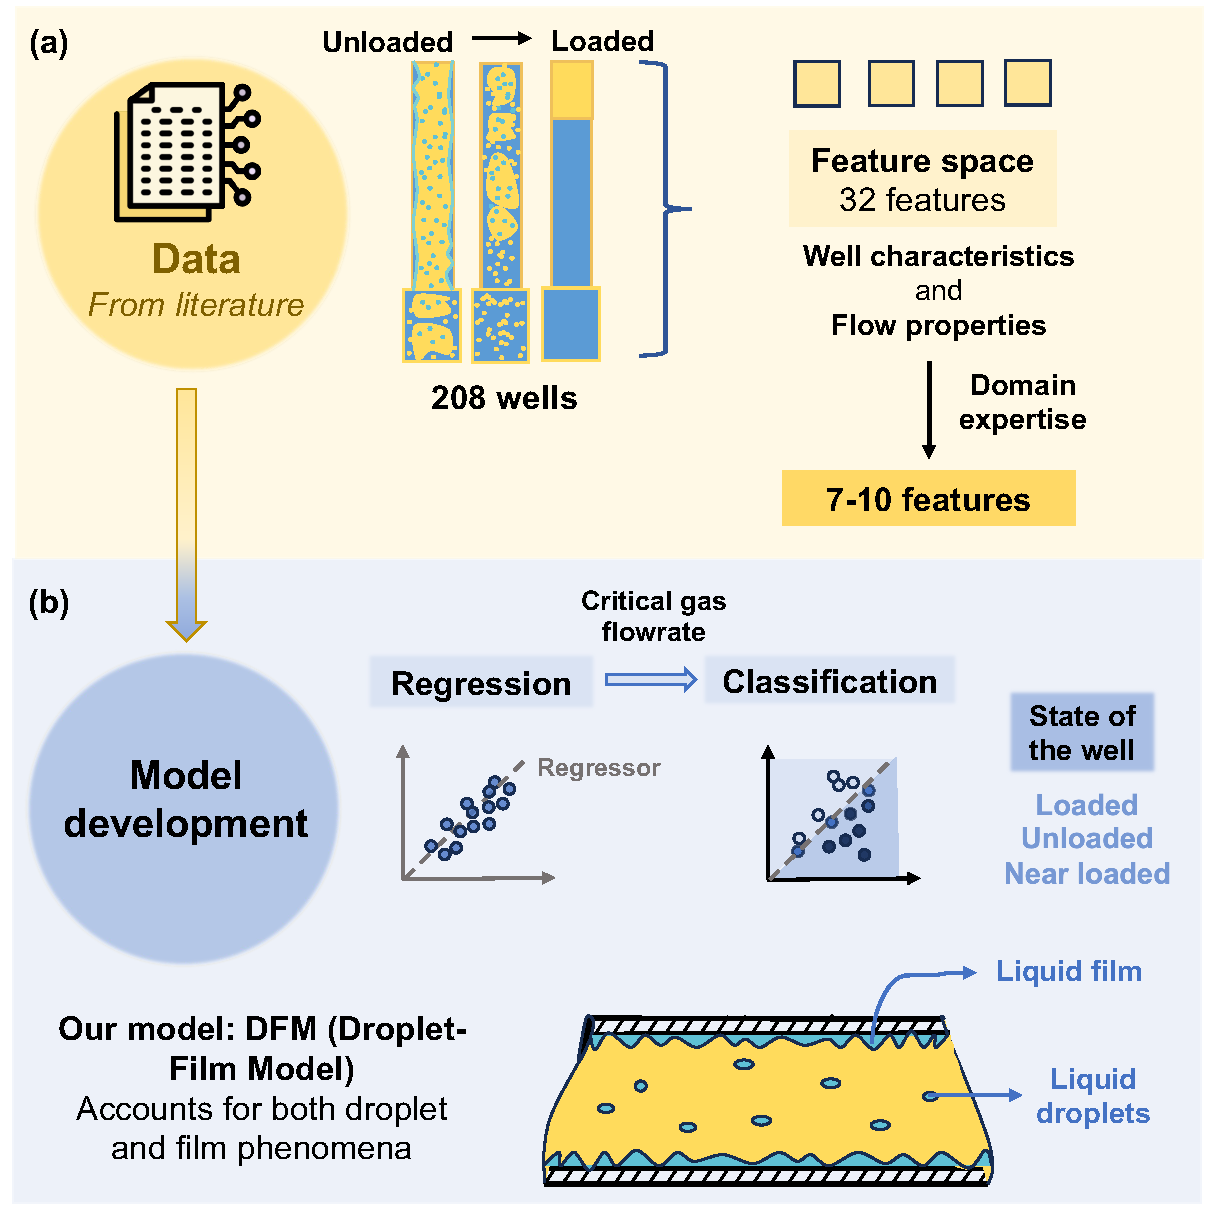
\includegraphics[width=0.5\linewidth]{Figures/workflow_combined_v2.pdf}
    \caption{Workflow of the present study: (a) data compilation and feature engineering, in which literature data from 208 gas wells were curated to construct a set of 32 candidate features and subsequently reduced to 7–10 key features using domain knowledge; (b) model development, involving a physics-based critical gas flow rate with a learned residual, followed by classification of wells as unloaded or loaded (near-loaded wells are shown on the cross plots and counted as loaded). The final framework integrates liquid film and droplet transport mechanisms and is referred to as the Droplet–Film Model.}
    \label{workflow}
\end{figure}

\al{The 16 wells with uncertain status were excluded, leaving 192 wells. Because only six wells are near-loaded, too few to learn this class reliably, the near-loaded wells were withheld from training entirely and used only for testing. The 186 loaded and unloaded wells were divided by a stratified 80--20 train-test split, giving 148 training wells and a test set of 44 wells (23 unloaded, 15 loaded, and all 6 near-loaded wells). The training set was used for model fitting and for hyperparameter selection through 5-fold stratified cross-validation (CV).}

\al{The DFM (and its single-mechanism variants) provides a critical gas flow rate, $\hat Q_{\text{critical}}$, for every well, as shown in eq. (\ref{eq:regression}), where $\bar X$ denotes the well features. QLattice and TabPFN are trained as classifiers of the probability that a well is unloaded, using the operating gas rate and the well features as inputs, and a well is predicted unloaded when this probability, evaluated at its operating rate, exceeds 0.5. For these models, an implied critical rate can be defined as the gas rate at which the probability equals 0.5 with all other features held fixed; however, as discussed in Section \ref{sec:results}, it does not exist for many wells. Because the true critical rate is never measured for any well, no model is fitted to a critical-rate target; all models are supervised only by the observed well status.} \al{For the DFM,} the predicted critical rate was compared with the operating gas flow rate to determine the well's loading state as loaded (1), unloaded ($-$1), and near-loaded (0), according to eq. (\ref{eq:class}). \al{Because gas rates in the dataset span two orders of magnitude, the near-loaded band is defined relative to the critical rate, using the log ratio of the two rates with $\epsilon = 0.05$ (i.e., within approximately $\pm 5\%$ of $\hat Q_{\text{critical}}$).}

\begin{equation}
\hat Q_{\text{critical}} = f(\bar X)
\label{eq:regression}
\end{equation}

\begin{equation}
\hat y =
\begin{cases}
1 & \text{if } \ln\left(Q_{\text{operating}}/\hat Q_{\text{critical}}\right) < -\epsilon \\
0 & \text{if } \left\lvert \ln\left(Q_{\text{operating}}/\hat Q_{\text{critical}}\right) \right\rvert \leq \epsilon \\
-1 & \text{if } \ln\left(Q_{\text{operating}}/\hat Q_{\text{critical}}\right) > \epsilon
\end{cases}
\label{eq:class}
\end{equation}


We computed the classification accuracy score of the model by comparing the predicted well status to the actual well status. This accuracy score was used for hyperparameter optimization during the 5-fold cross-validation. After selecting the optimal set of hyperparameters, the model was retrained on the entire training set and then tested on the \al{held-out test set of 44 wells. Because they are at risk of loading, the six near-loaded wells are counted as loaded in every accuracy (both as true labels and as predictions). They keep their own symbol only on the cross plots.}

\subsection{Modeling Approaches}
To systematically investigate the trade-offs among physical fidelity, interpretability, and predictive flexibility, we develop and compare three modeling approaches spanning from first-principles physics to fully data-driven learning. Firstly, we consider a physics-based model that explicitly incorporates liquid droplet \al{and liquid film} transport mechanisms, thereby embedding established mechanistic descriptions of the governing flow and transport processes\al{, augmented with a learned residual correction for effects not captured by the closed-form expression}. 

We also use a closed-form symbolic machine learning framework based on physical principles. Rather than prescribing functional forms \textit{a priori}, this method (QLattice) learns analytical expressions directly from data while enforcing consistency with known physical principles, thereby balancing interpretability with representational flexibility.\cite{Christensen2022QLattice} 

Lastly, we employ a black-box machine-learning model called TabPFN, which infers system behavior directly from data without explicit physical assumptions.\cite{kaplan2020scaling} By evaluating all three modeling approaches, this comparison enables a systematic assessment of the relative strengths and limitations of physics-based, physics-informed, and purely data-driven approaches for liquid loading prediction.

\subsubsection{Physics Informed Model development: Droplet Film Model (DFM)}
We developed a closed-form model that combines the LDM- and LFM-based approaches for liquid loading in gas wells. This model is termed the Droplet-Film Model (DFM). To develop this approach, we first derive the liquid droplet model through a force balance involving weight, drag, and buoyancy. This approach captures variations in droplet shape and other dynamic processes, such as the merging of two droplets into larger formations and the fragmentation of larger droplets into smaller ones. Through this approach, we derived the droplet critical velocity, shown in eq. (\ref{eq:droplet_only}). 

\begin{equation}
U_{\mathrm{droplet,crit}} = \frac{\left( \sin (p_1 \, \theta)\right)^{p_2}}{p_3} \left[ \frac{\sigma \, (\rho_l - \rho_g)^{p_4}}{\rho_g^2} \right] 
\label{eq:droplet_only}
\end{equation}
where \( \theta \) is the deviation angle in degrees, \( \rho_l \) and \( \rho_g \) are the densities (kg/m³) of liquid and gas, and $\{ q_i \}_{i \in \{1,2,3,4\}}$ represent XXX, which we recasted as learnable model parameters. 

To model the formation and changes of the liquid film along the wellbore, we formulated a momentum balance for the fluid, shown in the  \hl {SI subsection film only}. Specifically, the momentum equation describes how the net force acting on a section of the wellbore fluid relates to the rate of change of fluid momentum, providing a basis for estimating shear stresses at the pipe wall and within the flowing film \cite{OKORO20192443, LANDJOBOPAGOU2020103641}. Introducing a correction factor $\mathrm{C}_{f_1}$ to address issues with non-idealities in the film topography, we derived the film critical velocity, shown in eq. (\ref{eq:film}) 

\begin{equation}
U_{{\mathrm{film,\,crit}}} = \mathrm{C}_{f_1} \, \sqrt{\frac{2 \, g \, \delta \, (1 - 3 \bar{\delta} + 3 \bar{\delta}^2) \, (\rho_l - \rho_g) \, \cos \theta}{f_i \, \rho_g}},
\label{eq:film}
\end{equation}
where \( \delta \) is the film thickness (m), \( \bar{\delta} \) is the dimensionless film thickness, $g$ is the acceleration due to gravity (m/s²), \( \theta \) is the deviation angle in degrees, and \( f_i \) is the friction factor.  

The DFM model is then obtained by combining the expressions for the LDM, shown in eq. (\ref{eq:droplet_only}) and the LFM, shown in eq. (\ref{eq:film}). A mixing weight $\alpha \in [0, 1]$ is introduced so that the film mechanism dominates fully when $\alpha = 1$, the droplet mechanism dominates fully when $\alpha = 0$, and both contribute when $0 < \alpha < 1$. The critical velocity from the combined model is shown in eq. (\ref{eq:combined}). Although $\alpha$ may be written $\alpha(\theta)$ to indicate that the mix can depend on wellbore deviation, a single global $\alpha$ is fitted (see below); the well-wise, angle-dependent contribution of each mechanism is then evaluated with the film share (eq. (\ref{eq:film_share})).

\begin{equation}
U_{\mathrm{combined,\,crit}} 
= \alpha\, U_{\mathrm{film,\,crit}}\
+ \bigl(1 - \alpha\bigr)\, U_{\mathrm{droplet,\,crit}}
\label{eq:combined}
\end{equation}

Lastly, we used the derived $U_{\mathrm{combined,\,crit}}$ to compute the critical gas flow rate, $Q_{\mathrm{combined,\,crit}} $ via eq. (\ref{eq:combined2}).  A correction, $C_{f_2}$, is added to the learnable model parameters, which accounts for the physical phenomena that are not sufficiently captured by the original relationship and the underlying assumptions. 

\begin{equation}
Q_{\mathrm{combined,\,crit}} 
= 2.5 \times 10^{8}\,
\frac{C_{f_2}\, U_{\mathrm{combined,\,crit}}\, A\, P}
{z\, T},
\label{eq:combined2}
\end{equation}
where \textit{A} is the wellbore area (m$^2$), \textit{z} is the gas compressibility factor, \textit{T} is the wellbore temperature (K), and \textit{P} is the pressure (Pa).

\al{Altogether, the physics part of the DFM entails the learnable parameters $p_1$, $p_2$, $p_4$, $C_{f_1}$, $C_{f_2}$, and a single global mixing parameter $\alpha \in (0,1)$; the droplet prefactor $p_3$ cannot be identified separately from $C_{f_2}$ and $\alpha$ and is absorbed into them. Because the true critical rate is unknown, these parameters cannot be fitted by minimizing a regression error against $Q_{\text{critical}}$. Instead, they were estimated from the observed well status by minimizing a logistic (cross-entropy) loss on the classification margin $m = \ln(Q_{\text{operating}}/Q_{\text{combined,crit}})$, so that unloaded wells are pushed to $m>0$ and loaded wells to $m<0$. The loss was minimized with differential evolution in SciPy. The mixing weight was parameterized as $\alpha = \sigma(a)$, where $\sigma$ is the logistic function and $a$ is a free parameter; the fit gave $a = -6$ (the lower bound of the search range) and thus $\alpha = 0.0025$. A single global $\alpha$ was used rather than a per-well or $\alpha(\theta)$ form, so that the model can be evaluated for unseen wells without reference to their status. Replacing the global $\alpha$ by $\alpha(\theta) = \sigma(a_0 + a_1\cos\theta)$ collapsed to $\alpha \approx 0$ and did not improve accuracy, so the global value was retained. The relative contribution of the film and droplet mechanisms still varies from well to well through the angle-dependent terms $U_{\mathrm{film,crit}}$ and $U_{\mathrm{droplet,crit}}$, which is quantified by the film share in Section \ref{sec:results}.}

\al{To account for physical effects that are not captured by the closed-form expression, the DFM further learns a residual correction to the physics-based critical rate in log space:}
\begin{equation}
\ln \hat Q_{\text{critical}}^{\text{DFM}} = \ln Q_{\text{combined,crit}} + b + \mathbf{w}^{\top}\tilde{\mathbf{x}},
\label{eq:residual}
\end{equation}
\al{where $\tilde{\mathbf{x}}$ contains the standardized logarithms of $D$, $z$, $\rho_g$, $\rho_l$, $P/T$, $f_i$, and $\delta_{\text{crit}}$, together with $\cos\theta$ and $\sin\theta$. The intercept $b$, the weights $\mathbf{w}$, and the slope of the logistic link were fitted with the same logistic loss using L-BFGS-B, with an L2 penalty on $\mathbf{w}$ whose strength ($\lambda = 0.1$) was selected by 5-fold CV. The residual multiplies the physics-based critical rate by a well-specific factor $\exp(b + \mathbf{w}^{\top}\tilde{\mathbf{x}})$; it does not alter the relative contribution of the film and droplet terms. Details are given in the Supplementary Information.}

\subsubsection{Physics-Informed Symbolic Learning: QLattice}
QLattice is a symbolic regression framework designed to discover compact and interpretable mathematical expressions that accurately represent relationships observed in data \cite{Christensen2022QLattice}. In contrast to conventional regression techniques and black-box machine-learning models, QLattice explicitly searches the space of analytical expressions, producing closed-form equations. This approach enables physical interpretation of the learned models and facilitates insight into the underlying mechanisms governing the system behavior. 

The model construction process in QLattice is formulated as a probabilistic graph-based search, where candidate expressions are represented as computational graphs. The search is guided by Bayesian principles and information-theoretic criteria that balance predictive accuracy against model complexity, thereby discouraging overfitting and favoring parsimonious representations \cite{lundberg2020simple}. By iteratively refining and sampling expressions according to their posterior likelihood, QLattice efficiently explores a vast hypothesis space while retaining only those functional forms that achieve an optimal trade-off between explanatory power and simplicity. This makes QLattice particularly well-suited for physics-informed modeling, where interpretability, robustness, and consistency with known physical structure are essential.

\al{In this work, QLattice was used in classification mode to model the probability that a well is unloaded from the natural logarithm of the operating gas rate and the features $D$, $\theta$, $z$, $\rho_g$, $\rho_l$, $P/T$, $f_i$, and $\delta_{\text{crit}}$. A query constraint required $\ln Q_{\text{operating}}$ to enter every candidate expression additively, so that each discovered model is monotonic in the gas rate and yields a closed-form implied critical rate (the gas rate at which the predicted probability equals 0.5). Models were sampled for 20 epochs with a maximum complexity of 7 and ranked by the Bayesian information criterion. The QLattice model complexity is related to the number of edges in the resulting model graph, which controls the total number of features or interactions.}

\subsubsection{Black-Box Machine-Learning Model: Tabular Prior-Data Fitted Network (TabPFN) }
TabPFN is a transformer-based model pretrained on a large distribution of synthetic tabular datasets to approximate Bayesian posterior inference, enabling it to perform inference on new datasets in a single forward pass. By conditioning directly on the provided training samples, it leverages in-context learning in transformer models \cite{kaplan2020scaling} and produces predictions for unseen data without iterative training or extensive hyperparameter tuning. Unlike traditional models that learn explicit parametric relationships, TabPFN leverages contextual attention mechanisms to adapt its predictions to the structure of the dataset at hand. This allows it to capture complex interactions between features and respond flexibly to class imbalance and regime changes, which are common in real-world engineering datasets. As a result, TabPFN is particularly well-suited for problems where the available labeled data are limited and heterogeneous, as is often the case in wellbore and production-related applications\cite{TabPFN-2.5}. \al{Here, the TabPFN classifier was given the natural logarithm of the operating gas rate together with the ten well features and was used with its default settings. TabPFN does not provide an explicit expression for the critical rate. Wells were therefore classified directly from the predicted probability of the unloaded class at the measured gas rate (unloaded if this probability exceeds 0.5).}

\section{\textbf{Results and discussion}}\label{sec:results}

\subsection{Model Performance and Comparison}
\label{sec:results_nlpesr}
\al{The DFM achieved a CV classification accuracy of 85.8\% ($\pm$3.5\%) and a test accuracy of 90.9\%. The QLattice model achieved a CV accuracy of 82.4\% ($\pm$5.2\%) and a test accuracy of 88.6\%. The discovered expression, eq. (\ref{eq:qlattice_new}), gives the probability that a well is unloaded; setting this probability to 0.5 yields the closed-form implied critical rate in eq. (\ref{eq:qlattice_qcr}). The implied critical rate increases steeply with the critical film thickness $\delta_{\text{crit}}$ and decreases with the interfacial friction factor $f_i$, consistent with the film model, in which a thicker film requires more gas momentum to lift and a larger interfacial friction transfers that momentum more effectively. Lastly, the black-box TabPFN model achieved the highest CV accuracy, 91.8\% ($\pm$4.7\%), with a test accuracy of 84.1\%, as shown in Figure \ref{class_acc}. Thus, while TabPFN fits the training distribution best, the three models generalize similarly to the held-out test wells (84--91\%), and the gap between TabPFN's CV and test accuracy suggests some overfitting given the small dataset.}

\begin{equation}
P(\text{unloaded}) = \sigma\!\left(0.22 \ln Q_{\text{operating}} - 1.22 \ln\left(4300\,\delta_{\text{crit}} - 65.2\, f_i + 0.02\right) - 4.92\right)
\label{eq:qlattice_new}
\end{equation}

\begin{equation}
\hat Q_{\text{critical}}^{\text{QLattice}} = 5.2 \times 10^{9} \left(4300\,\delta_{\text{crit}} - 65.2\, f_i + 0.02\right)^{5.55}
\label{eq:qlattice_qcr}
\end{equation}
\al{where $\sigma(\cdot)$ is the logistic function, $\delta_{\text{crit}}$ is in m, and the rates are in m$^3$ day$^{-1}$.}

\begin{figure}[!t]
    \centering
    \captionsetup{width=0.89\textwidth}
    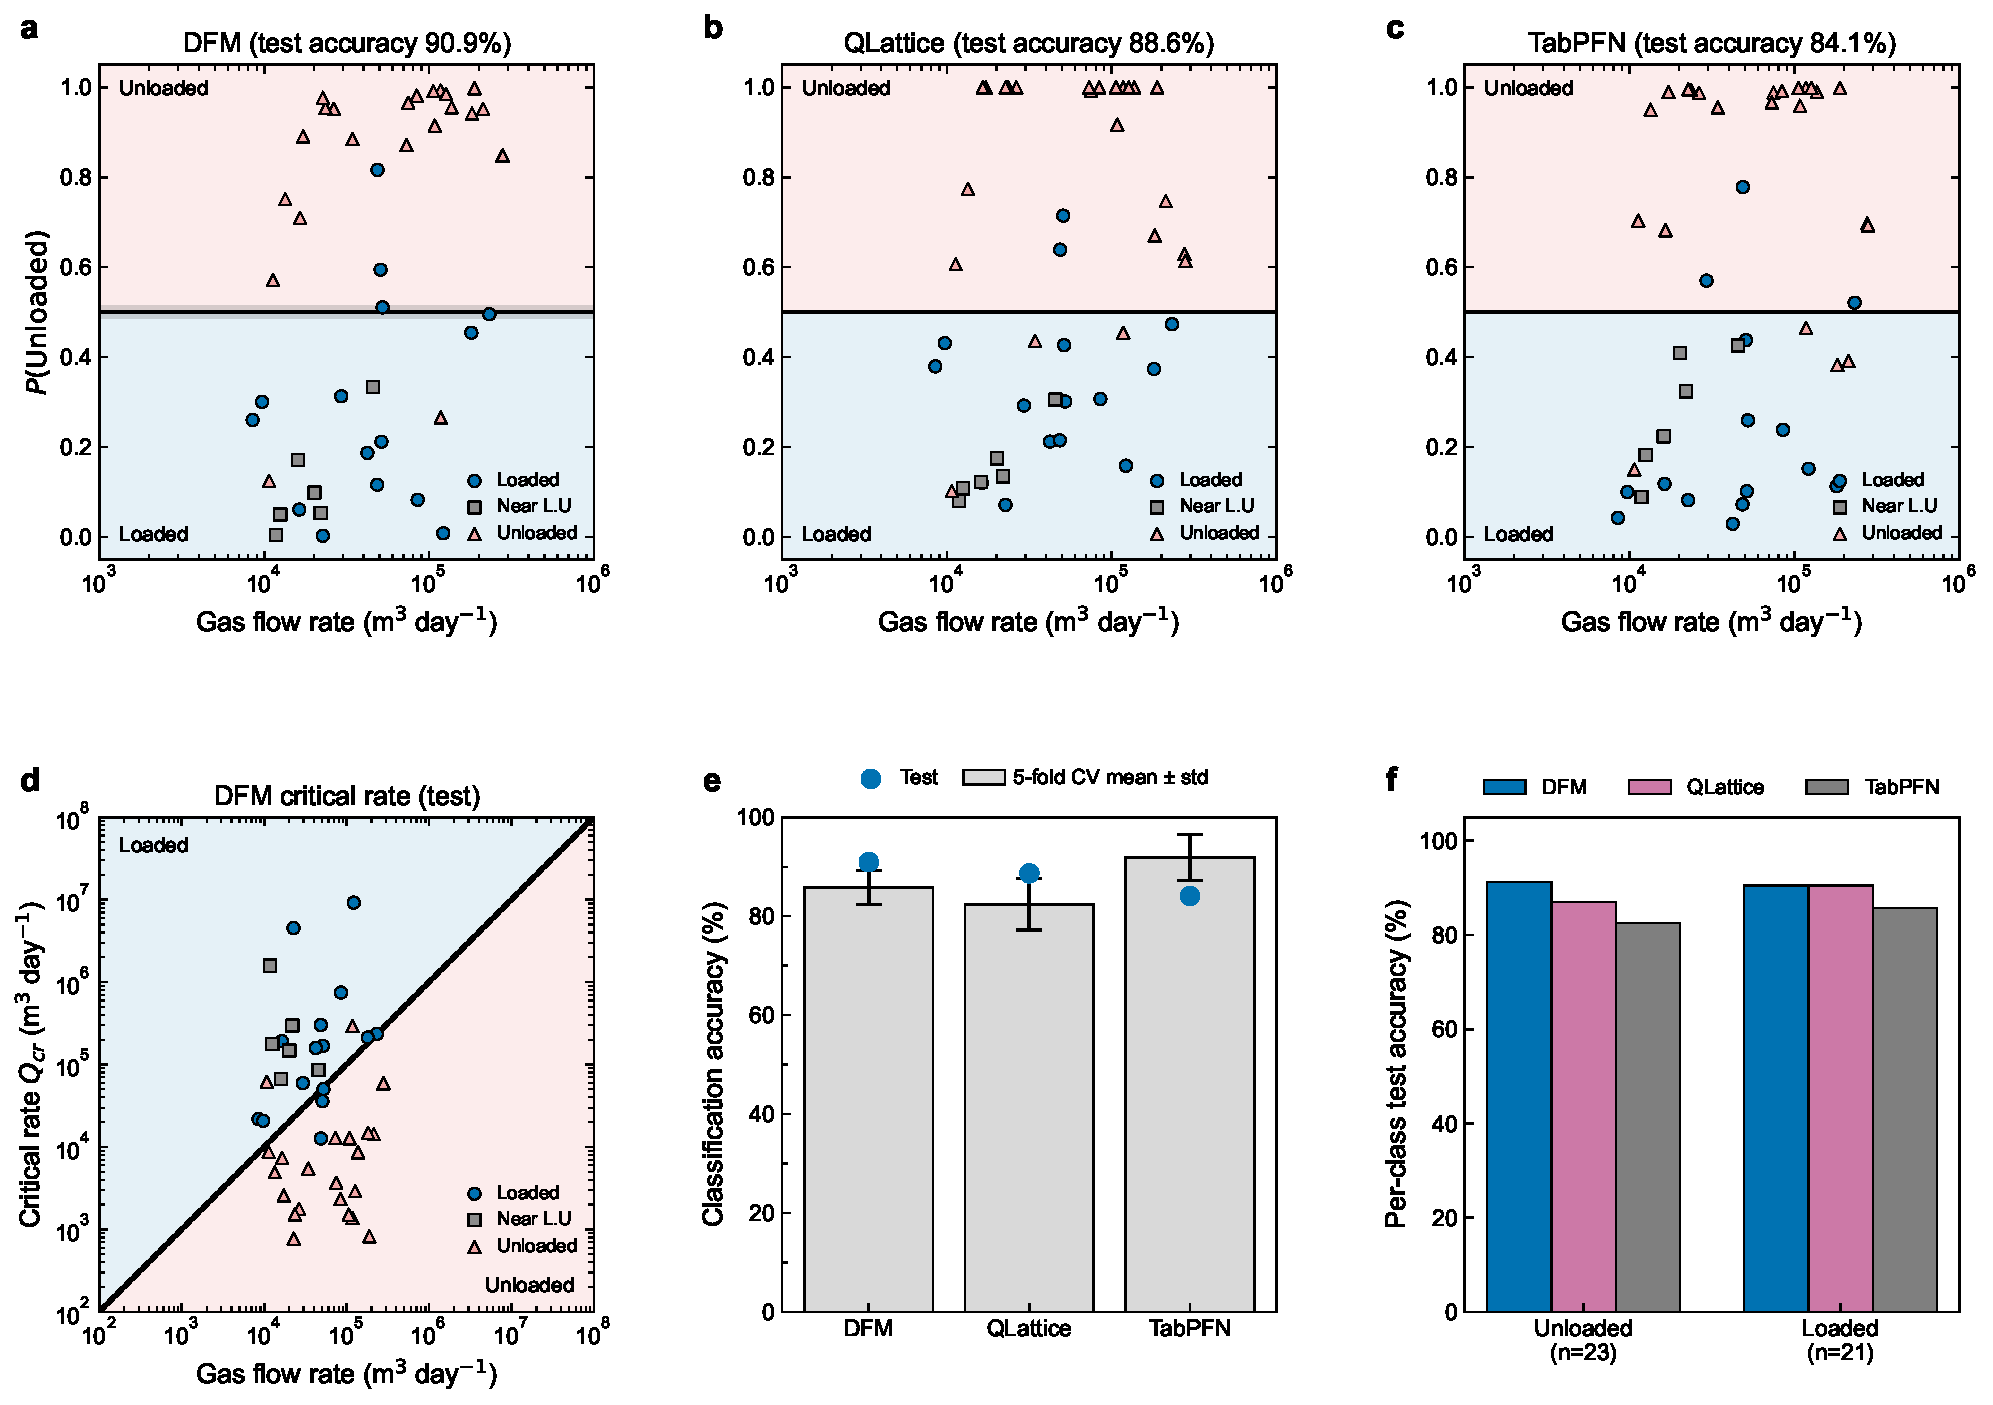
\includegraphics[width=0.98\linewidth]{Figures/figure2_updated.pdf}
    \caption{\al{Results for the 44 test wells. (a--c) Predicted probability that a well is unloaded at its observed gas flow rate for the DFM (a), QLattice (b), and TabPFN (c); the black line marks the 0.5 decision threshold, and the gray strip in (a) marks the DFM near-loaded band. (d) DFM critical flow rate versus observed gas flow rate; the dashed lines bound the $\pm$5\% near-loaded band. In (a)--(d), blue circles are loaded, gray squares near-loaded (Near L.U.), and pink triangles unloaded wells. (e) Classification accuracy: 5-fold CV (bars, mean $\pm$ standard deviation) and test accuracy on the 44 wells (circles). (f) Per-class test accuracy on the unloaded and loaded wells.}}
    \label{class_acc}
\end{figure}

To analyze the relative performance of the models in classifying well loading, we compared the models \al{in Figure \ref{class_acc}(a)--(d). Panels (a)--(c) show, for each model, the predicted probability that a well is unloaded at its measured gas flow rate, and panel (d) compares the DFM critical flow rates to the measured gas flow rates.} Please note that the flow rate in the figures refers to the gas production rate of the well at the specific instant at which it is evaluated to determine whether liquid loading has occurred. This flow rate is measured under controlled or diagnostic operating conditions and is used as a reference point for assessing the well’s loading status.

\al{To compare the three models one-to-one, Figure \ref{class_acc}(a)--(c) shows the same quantity for each: the predicted probability that a well is unloaded, with the decision threshold at 0.5. QLattice and TabPFN predict only this probability, and an implied critical rate does not exist for many wells (see below). The DFM is trained with a logistic loss, so its probability follows directly from its critical rate, $\sigma(k \ln(Q_{\text{operating}}/\hat Q_{\text{critical}}))$ with the learned slope $k = 1.11$. It is therefore equivalent to the critical-rate classification, and the $\pm$5\% near-loaded band becomes the thin strip around 0.5 in panel (a). In addition, the DFM provides the critical rate itself for every well (panel d): wells above the diagonal, where the predicted critical rate exceeds the operating rate, are predicted as loaded, and wells below it as unloaded. All test wells lie within the axes of every panel. Near-loaded wells are shown with their own symbol on the cross plots and, as described in Section \ref{sec:method}, are counted as loaded in every accuracy. In probability space, the DFM assigns less extreme probabilities than QLattice and TabPFN, which place most unloaded wells close to 1, reflecting the gradual transition between the classes learned by the DFM (SI). The DFM produces a continuous spread of critical rates around the threshold line, with loaded wells mostly above and unloaded wells mostly below it. It misclassifies two of the 23 unloaded wells as loaded and two of the 21 loaded wells as unloaded; two further loaded wells fall in the near-loaded band on the cross plot and are counted as loaded. The QLattice model misclassifies three unloaded wells as loaded and two loaded wells as unloaded, and TabPFN misclassifies four unloaded and three loaded wells (Figure \ref{class_acc}(b,c)). However, neither model yields a usable critical rate for every well. The QLattice expression for the critical rate, eq. (\ref{eq:qlattice_qcr}), is undefined for 12 of the 44 test wells (62 of all 192 wells), for which $4300\,\delta_{\text{crit}} - 65.2\, f_i + 0.02 \le 0$, and where it is defined it spans implausible values, from about $10^{-5}$ to $10^{9}$~m$^3$/day. For TabPFN, the predicted probability of the unloaded class changes so weakly with the gas rate that, for 29 of the 44 test wells, it does not cross 0.5 anywhere between $10^{-6}$ and $10^{6}$ times the measured rate. These models therefore separate the classes well, mainly through the well features rather than the gas rate, but do not provide physically meaningful critical-rate estimates, in contrast to the DFM.}

\al{The per-class accuracies in Figure \ref{class_acc}(f) confirm that the three models perform similarly on the two classes: the DFM achieves the highest accuracy on unloaded wells (91.3\%, compared with 87.0\% for QLattice and 82.6\% for TabPFN) and matches QLattice on loaded wells (90.5\%, compared with 85.7\% for TabPFN). All three models place all six near-loaded wells in the loaded region. None of them falls inside the $\pm$5\% near-loaded band: their operating rates lie between roughly 1\% and 50\% of the DFM critical rate, so the models cannot distinguish them from loaded wells given the available features, but they do flag them as at risk of loading. Overall, DFM attains classification accuracy comparable to the data-driven approaches while additionally offering physical interpretability (discussed below).}
\begin{figure}[H]
    \centering
    \captionsetup{width=0.89\textwidth}
    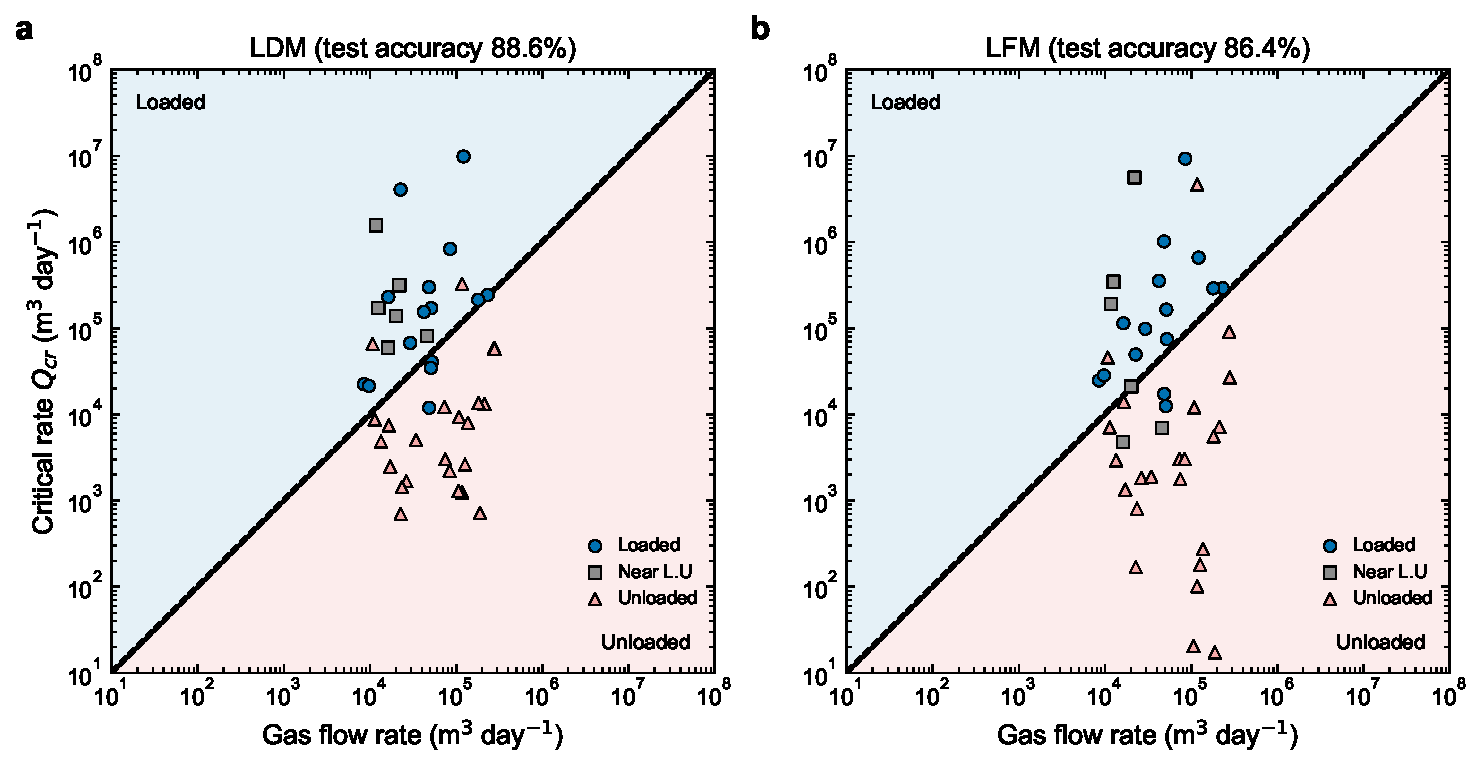
\includegraphics[width=0.89\linewidth]{Figures/figure3_updated.pdf}
    \caption{Predicted critical flow rates versus observed flow rates for \al{the 44 test wells} using the LDM model \al{(a)} and LFM model \al{(b), both fitted within the DFM framework with the film or droplet term zeroed out, respectively}. Points are colored by true well condition: blue circles (Loaded), gray squares (Near load Up), and pink triangles (Unloaded). The diagonal black line represents the ideal prediction threshold where predicted critical rate equals observed flow rate; points above the line are predicted as loaded, while points below are predicted as unloaded, and the dashed lines enclosing the gray region correspond to the near-loaded \al{band ($\pm$5\% of the critical rate). All test wells lie within the axes.}}
    \label{fig3}
\end{figure}

We also compared the performance of LDM, LFM, and DFM using cross-plots as shown in \al{Figure \ref{fig3} and Figure \ref{class_acc}(d). The LDM and LFM were obtained within the same framework as the DFM, with the same loss, learned residual, data split, and classification rule, by zeroing out the film term ($\alpha = 0$, LDM) or the droplet term ($\alpha = 1$, LFM) in eq. (\ref{eq:combined}).}

\al{The LDM achieves a CV accuracy of 85.1\% ($\pm$3.6\%) and a test accuracy of 88.6\% (91.3\% unloaded, 85.7\% loaded), close to the DFM (85.8\% $\pm$ 3.5\% and 90.9\%; 91.3\% unloaded, 90.5\% loaded). The LFM has a lower CV accuracy, 81.1\% ($\pm$4.6\%), and a test accuracy of 86.4\% (91.3\% unloaded, 81.0\% loaded). The DFM and LDM place all six near-loaded wells in the loaded region, whereas the LFM places two of them in the unloaded region. Given the size of the test set, these test differences correspond to one or two wells and are within the variability indicated by the CV standard deviations. The close agreement between the LDM and the DFM is expected, because the fitted DFM mixing parameter is small ($\alpha = 0.0025$; see also the film share in eq. (\ref{eq:film_share}) and Figure \ref{alpha_dev}) and the DFM is therefore close to droplet-only. The value of combining both mechanisms in the DFM lies mainly in the mechanistic interpretation discussed below.} 

\subsubsection*{\al{Film Share Analysis}: Identifying Dominant Flow Mechanisms Across Wellbore Deviations}

\al{Because the DFM uses a single global $\alpha$, the value of $\alpha$ alone does not indicate which mechanism dominates in a given well; moreover, the film and droplet terms differ in magnitude by orders of magnitude, so $\alpha$ mainly acts as a scale balance between them. We therefore quantify the dominant mechanism for each well by the film share. After the physics parameters and $\alpha$ have been fitted on the training wells, $U_{\mathrm{film,crit}}$ and $U_{\mathrm{droplet,crit}}$ are evaluated at each well's features from eqs.\ (\ref{eq:film}) and (\ref{eq:droplet_only}). The same fitted $\alpha$ then weights the two terms as in eq. (\ref{eq:combined}), and the film share is}
\begin{equation}
\phi_{\text{film}} = \frac{\alpha\, U_{\mathrm{film,crit}}}{\alpha\, U_{\mathrm{film,crit}} + (1-\alpha)\, U_{\mathrm{droplet,crit}}},
\label{eq:film_share}
\end{equation}
\al{i.e., the fraction of the combined critical velocity contributed by the film mechanism. Variation in $\phi_{\text{film}}$ across wells comes only from the well features, mainly $\theta$ through $\cos\theta$ in the film term and $\sin(p_1\theta)$ in the droplet term; $\alpha$ itself is held fixed at the fitted value $0.0025$. A value of $\phi_{\text{film}} = 0$ indicates a purely droplet-controlled critical rate, $\phi_{\text{film}} = 1$ a purely film-controlled one, and $\phi_{\text{film}} > 0.5$ a film-dominated well. The residual correction of eq. (\ref{eq:residual}) multiplies the whole critical rate after this combination and does not enter eq. (\ref{eq:film_share}), so the film-share map is a property of the physics part of the DFM only. Figure \ref{alpha_dev} reports $\phi_{\text{film}}$ for all 192 wells using the parameters fitted on the 148 training wells.}

\al{The distribution of $\phi_{\text{film}}$ with wellbore deviation angle is shown in Figure \ref{alpha_dev}. The droplet term dominates the critical rate at all deviation angles represented in the dataset (20--90$^\circ$): only 3 of 192 wells have $\phi_{\text{film}} > 0.5$. The film contribution is largest at low deviation angles (median $\phi_{\text{film}}$ of 30\% for 20--35$^\circ$, interquartile range 16--39\%, with those three wells exceeding 50\%), decreases to approximately 9--11\% at 35--75$^\circ$, and is identically zero for the 90 horizontal wells. The last of these follows directly from the film expression, eq. (\ref{eq:film}), in which $U_{\mathrm{film,crit}} \propto \sqrt{\cos\theta}$ vanishes at $\theta = 90^\circ$, so those wells carry no information on the film contribution. This is the reverse of the common expectation that liquid films dominate in horizontal wells; in this formulation the film term cannot contribute at $90^\circ$. The pattern was stable across the five cross-validation refits and under widened parameter bounds. The dataset contains no wells with deviation angles below 20$^\circ$, so the behavior of near-vertical wells cannot be assessed from these data.}

\begin{figure}[H]
\captionsetup{width=0.89\textwidth}
\centering
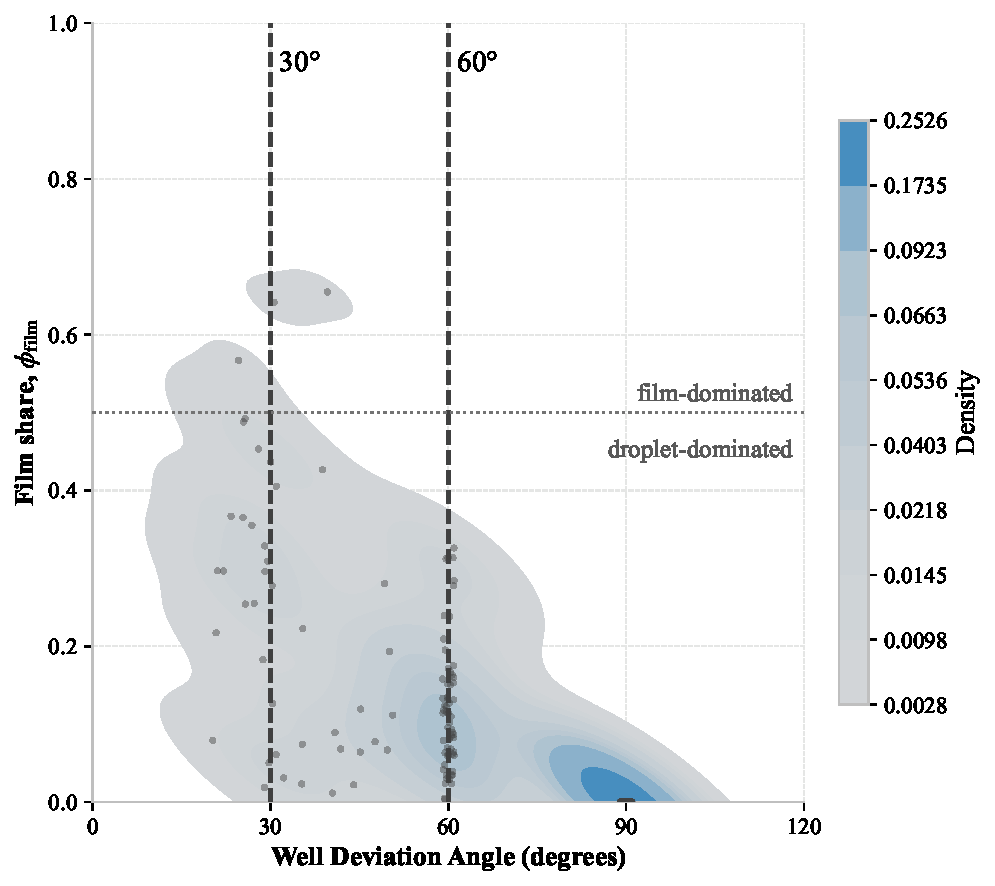
\includegraphics[width=0.5\textwidth]{Figures/film_share_vs_deviation.pdf}
\caption{\al{Joint distribution of the film share $\phi_{\text{film}}$ (eq. (\ref{eq:film_share})) and wellbore deviation angle for all 192 wells. For each well, $U_{\mathrm{film,crit}}$ and $U_{\mathrm{droplet,crit}}$ are evaluated from the fitted DFM physics parameters and combined with the same global $\alpha = 0.0025$. Values below 0.5 (dotted line) indicate droplet-dominated wells. Dots show individual wells; at 90$^\circ$, $\phi_{\text{film}} = 0$ by construction because $U_{\mathrm{film,crit}} \propto \sqrt{\cos\theta}$.}}
\label{alpha_dev} 
\end{figure} 
\mz{[Note for coauthors: in Figure \ref{comp_lit}, the literature bars are unchanged (Turner benchmark wells), while the DFM, QLattice, and TabPFN bars are now their accuracies on the 44 held-out test wells, so the two groups are evaluated on different wells. The per-well literature predictions are needed to put all models on the same wells. Near-loaded wells are now merged into the loaded class; for the literature models, the merged loaded accuracy is (loaded correct + near-loaded correct)/37, using the original counts (31 loaded + 6 near-loaded = 37, which resolves the earlier 37 vs.\ 31 discrepancy). If the original near-loaded counts only credited exact near-loaded predictions, the literature values are slightly conservative.]}

We compared the performance of the model studied in this work against existing analytical models through confusion matrix analysis. These existing models are typically derived from mechanistic formulations and can be broadly categorized as either droplet-based or film-based mechanisms for liquid loading. In contrast, the DFM model integrates both droplet and film contributions into a unified framework, allowing it to capture transitions between the two regimes. The  Turner et al\cite{Turner1969} dataset, which consists of 53 unloaded, 6 near-loaded, and 37 loaded wells, was used for this comparison because some of the mechanistic models compared were tuned with this dataset. In this study, it represents a subset of the original training and testing data used for model development and was chosen because it is commonly used for benchmarking models in the field of liquid-loading prediction. These models were also compared with the TabPFN and Qlattice models.

\begin{figure}[!t]
\captionsetup{width=0.89\textwidth}
\centering
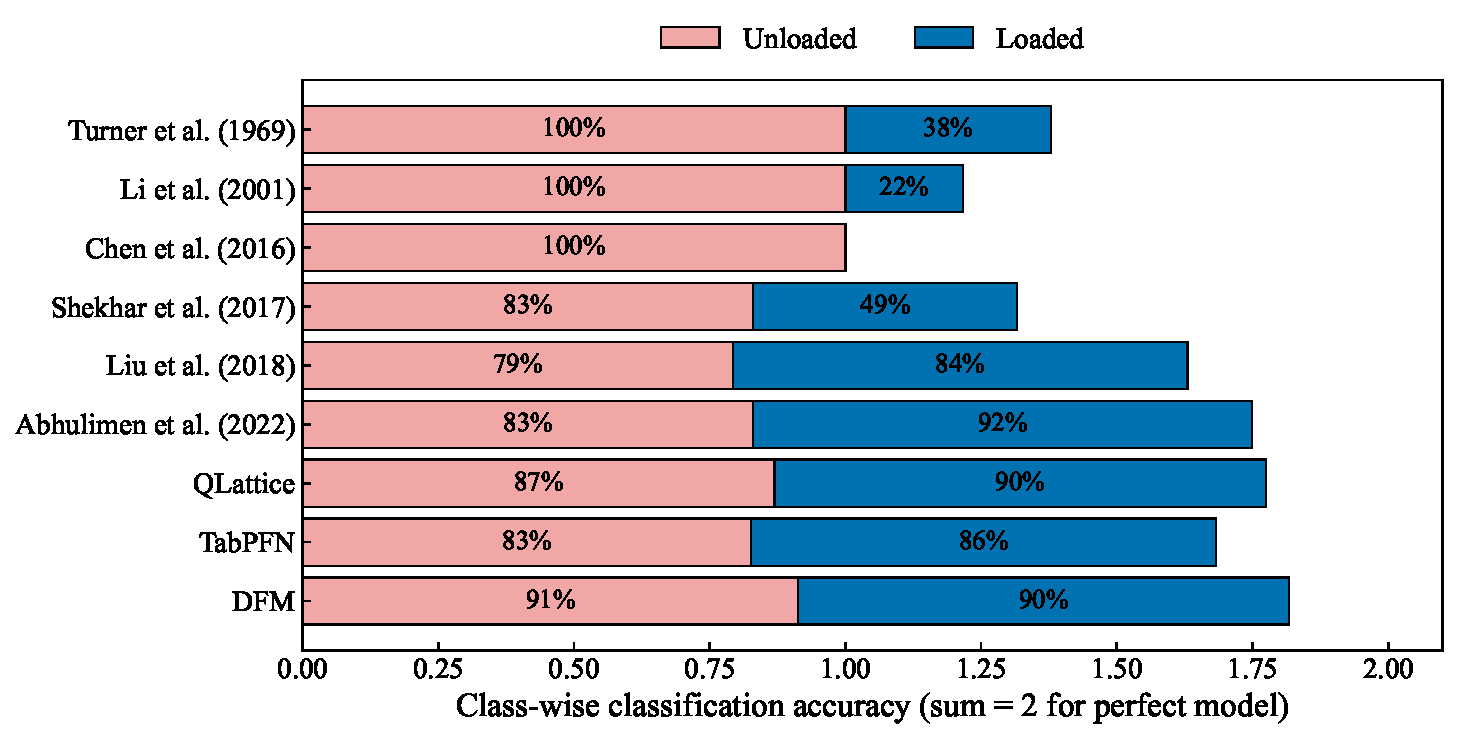
\includegraphics[width=0.85\textwidth]{Figures/stacked_classwise_accuracy_updated.pdf}
\caption{Class-wise classification accuracy for liquid loading identification in gas wells, comparing classical physics-based models from literature (Turner et al.\cite{Turner1969}; Li et al.\cite{Li2001}; Chen et al.\cite{Chen2016}; Shekhar et al.\cite{Shekhar}; Liu et al.,\cite{Liu2018}; Abhulimen et al.\cite{Abhulimen}), the Qlattice model, the TabPFN model, and the proposed DFM model. Each bar is segmented by true class: pink (Unloaded) and blue (Loaded\al{, including the near-loaded wells}). The x-axis represents summed class-wise accuracy (maximum \al{2.0} for a perfect model). \al{The literature models are evaluated on the Turner et al. benchmark wells (53 unloaded and 37 loaded or near-loaded wells); the QLattice, TabPFN, and DFM bars show their accuracy on the 44 held-out test wells of this study (23 unloaded and 21 loaded or near-loaded wells).}}
\label{comp_lit}
\end{figure}

 The data in Figure \ref{comp_lit} shows a comparison of class-wise classification performance between established physics-based critical rate models from the literature and the models evaluated in this study. Traditional models, such as Turner \textit{et al.} (1969)\cite{Turner1969}, Li \textit{et al.} (2001)\cite{Li2001}, and Chen \textit{et al.} (2016)\cite{Chen2016}, were developed primarily to predict the onset of liquid loading under specific assumptions and typically excel at identifying one regime (usually the unloaded or loaded state dominant in their training datasets) while exhibiting significant inaccuracies in the minority or transitional classes. This results in highly imbalanced summed accuracies, \al{at most 1.4 out of 2.0} despite appearing perfect on the targeted class. More recent correlations (e.g., Liu \textit{et al.}, 2018\cite{Liu2018}; Abhulimen \textit{et al.}, 2022\cite{Abhulimen}) show \al{a substantially better balance, with summed accuracies of 1.63 and 1.75.} \al{The three models developed in this study achieve similarly balanced accuracies on the held-out test wells: QLattice 87\% on unloaded and 90\% on loaded wells, TabPFN 83\% and 86\%, and the DFM 91\% and 90\%, with summed accuracies of 1.77, 1.68, and 1.82. They thus clearly outperform the classical correlations and perform on par with, or slightly above, the most recent correlation of Abhulimen \textit{et al.} (1.75). Among these balanced models, the DFM is the most accurate on unloaded wells and matches QLattice on loaded wells, while Abhulimen \textit{et al.} remain the most accurate literature correlation on loaded wells. Because the accuracies of the models of this study are computed on a different, smaller set of wells than those of the literature models, the comparison indicates the balance across classes rather than an exact ranking. The close performance between the interpretable DFM and the black-box TabPFN suggests that incorporating domain knowledge can yield predictive power comparable to state-of-the-art tabular learning methods. On the test wells, the DFM misclassifies two of the 23 unloaded wells as loaded and two of the 21 loaded wells as unloaded. Flagging wells near the loading boundary as loaded is the preferable error in a diagnostic setting, where a false alarm merely prompts additional verification, whereas a missed loading condition could lead to production losses.}

\section{Conclusion}\label{sec:conclusion}
We developed a physics-informed Droplet-Film model (DFM) that integrates droplet and film flow theories to overcome their individual limitations in predicting liquid loading conditions in gas wells. Exploratory data analysis revealed strong correlations between parameters governing both droplet and liquid film, and the critical velocity, motivating the need for a unified theoretical framework. We compared the performance of the DFM model against two data-driven approaches--the Qlattice symbolic regression model and the TabPFN tabular prior-fitted network. \al{Because the true critical rate is never measured, all models were trained directly on the observed well status, and the DFM includes a learned log-space residual. It achieved a cross-validation accuracy of 86\%. TabPFN achieved the highest cross-validation accuracy (92\%), but on the 44 held-out test wells the three models performed similarly (DFM 90.9\%, QLattice 88.6\%, TabPFN 84.1\%). The six near-loaded wells, withheld from training, are counted as loaded and are shown with their own symbol only on the cross plots; all three models place them in the loaded region, flagging them as at risk of loading, although none of the models resolves them as a separate class. The QLattice model yielded a compact closed-form critical rate governed by the critical film thickness and the interfacial friction factor, although this expression is undefined for about one third of the wells, whereas TabPFN provides no explicit expression and its predictions depend only weakly on the gas rate, so that no implied critical rate exists for most test wells. The DFM, in addition to matching the data-driven models in accuracy, provides insight into the dominant flow mechanism: the film share computed with the fitted global $\alpha$ shows that the droplet term dominates at all deviation angles in the data (20--90$^\circ$), with the film contribution largest at 20--35$^\circ$ (median 30\%) and identically zero in horizontal wells.} These findings indicate that physics-informed approaches like DFM offer \al{predictive performance comparable to purely data-driven models together with} advantages in interpretability and practical deployability. This balance makes DFM a viable and reliable option for the diagnosis and management of liquid loading in gas wells. This comparative analysis reveals that relying exclusively on a single theoretical framework is often insufficient, underscoring the importance of integrative, theory-informed modeling approaches.

%%===========================================================================================%%
%% If you are submitting to one of the Nature Portfolio journals, using the eJP submission   %%
%% system, please include the references within the manuscript file itself. You may do this  %%
%% by copying the reference list from your .bbl file, paste it into the main manuscript .tex %%
%% file, and delete the associated \verb+\bibliography+ commands.                            %%
%%===========================================================================================%%
\section{Supplementary Information}
(\href{SI.pdf}Supplementary information).
\section{Code availability}
All code and data used to develop the models and perform any analysis can be found at the following GitHub repository: \href{https://github.com/Awwal41/symbolic-machine-learning-liquidloading}{https://github.com/Awwal41/Droplet-Film-Theory-Development}

\bibliography{sn-bibliography}  % Put reference papers in the sn-bibliography.bib 
%% if required, the content of .bbl file can be included here once bbl is generated
%%\input sn-article.bbl

\newpage


\end{document}
